\section{Evaluación de la calidad del software}

Con el propósito de complementar la verificación funcional presentada en la sección anterior con una valoración de la calidad técnica del código fuente, se realizó un análisis estático del prototipo FLP Viewer mediante SonarCloud. Esta evaluación permite identificar problemas relacionados con confiabilidad, seguridad, mantenibilidad, duplicación de código y cobertura de las pruebas automatizadas, aspectos que no son observables a través de la verificación de requisitos funcionales descrita previamente.

SonarCloud es una plataforma de análisis continuo de código fuente que examina un proyecto en busca de errores (\textit{bugs}), vulnerabilidades, \textit{code smells}\footnote{Patrones de código que, sin constituir errores funcionales, incrementan la deuda técnica y dificultan el mantenimiento del software.} y fragmentos duplicados, además de integrar los resultados de cobertura generados por las pruebas automatizadas del proyecto. Sobre estas métricas, la plataforma aplica \textit{Quality Gates}, definidos como un conjunto de condiciones que se evalúan sobre los resultados de cada análisis para determinar si el código cumple un nivel mínimo de calidad. El \textit{Quality Gate} se reporta como aprobado cuando los resultados satisfacen dichas condiciones, y como no aprobado en caso contrario \cite{sonarcloud_quality_gates}.

Para la evaluación del prototipo, el repositorio de FLP Viewer se integró con SonarCloud y se ejecutó el análisis sobre la rama principal (\texttt{main}) una vez finalizado el desarrollo de las funcionalidades contempladas, con el propósito de obtener una medición del estado final del código. La Figura \ref{fig:sonarcloud} presenta el panel de resultados generado por la plataforma, y la Tabla \ref{tab:sonarcloud-resultados} resume los valores obtenidos para cada métrica.

\begin{figure}[H]
    \centering
    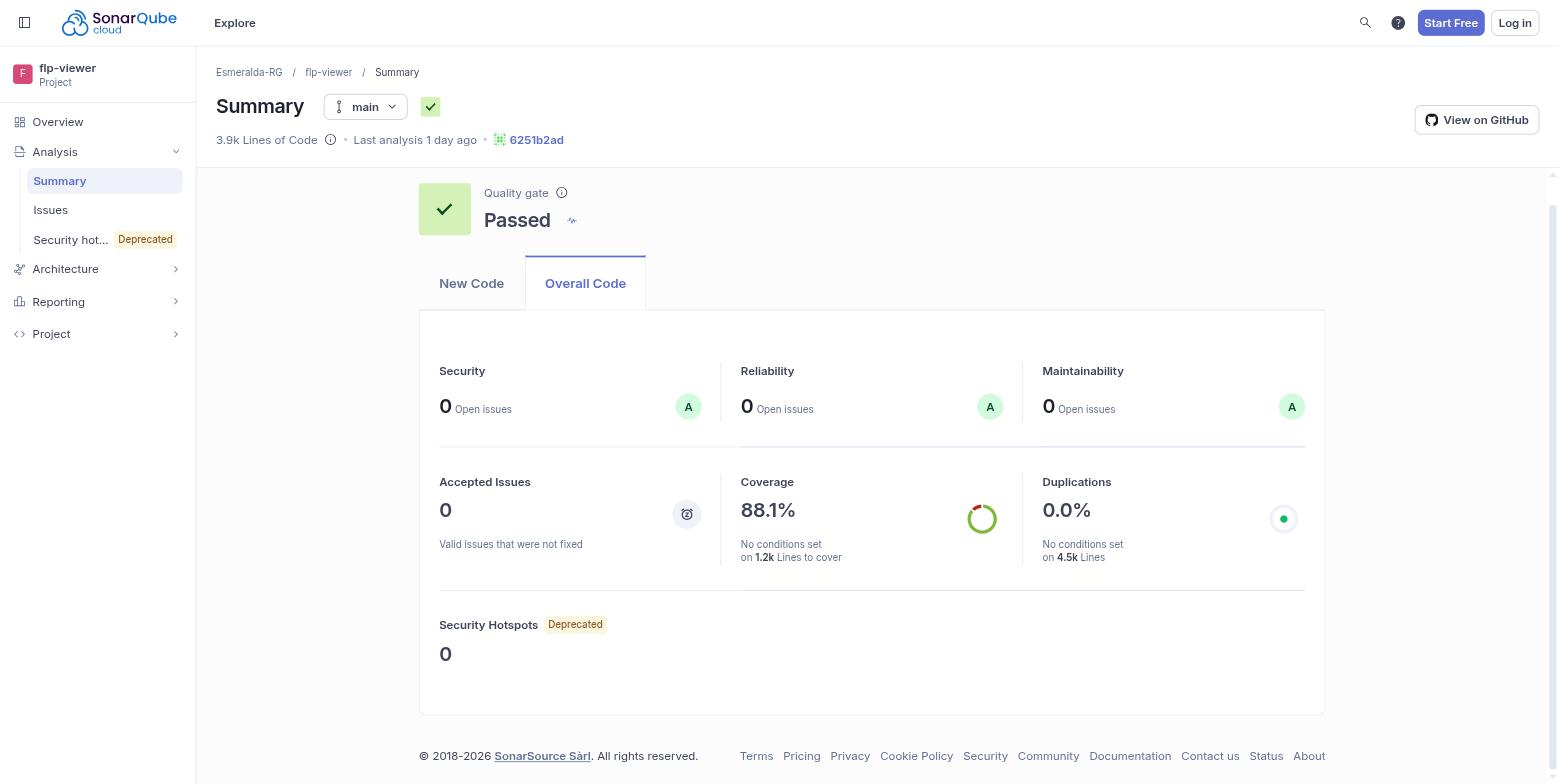
\includegraphics[width=0.85\textwidth]{Capitulo_5/imagenes/sonarcloud-resumen.jpg}
    \caption{Panel de resultados del análisis de calidad del prototipo FLP Viewer en SonarCloud}
    \scriptsize \textbf{Fuente:} SonarCloud, rama \texttt{main} del repositorio del proyecto
    \label{fig:sonarcloud}
\end{figure}

\begin{table}[H]
\centering
\footnotesize
\caption{Resultados del análisis de calidad del prototipo FLP Viewer mediante SonarCloud}
\label{tab:sonarcloud-resultados}
\begin{tabular}{|l|c|}
\hline
\textbf{Métrica} & \textbf{Resultado} \\
\hline
Quality Gate & Aprobado \\
\hline
Bugs & 0 \\
\hline
Vulnerabilidades & 0 \\
\hline
Code Smells & 0 \\
\hline
Security Hotspots & 0 \\
\hline
Duplicación de código & 0.0\,\% \\
\hline
Cobertura de código & 88.1\,\% \\
\hline
Reliability Rating & A \\
\hline
Security Rating & A \\
\hline
Maintainability Rating & A \\
\hline
\end{tabular}
\vskip 4pt
\footnotesize\textit{Fuente: elaboración propia, a partir del análisis de SonarCloud sobre la rama \texttt{main} del repositorio\footnote{\url{https://sonarcloud.io/summary/overall?id=Esmeralda-RG_flp-viewer&branch=main}}.}
\end{table}

La cobertura obtenida, del 88.1\,\%, indica la proporción del código ejecutable del prototipo que fue ejercitada mediante las pruebas automatizadas del proyecto. Esta métrica permite identificar qué partes del código fueron efectivamente recorridas durante las pruebas y, en consecuencia, detectar zonas que podrían requerir casos de prueba adicionales \cite{sonarcloud_coverage}. Las calificaciones de confiabilidad, seguridad y mantenibilidad obtenidas corresponden en los tres casos al nivel A, el más favorable de la escala empleada por SonarCloud, en la cual el nivel A de confiabilidad y de seguridad se asigna cuando el análisis no reporta errores ni vulnerabilidades, respectivamente, y el nivel A de mantenibilidad se asigna cuando la deuda técnica estimada no supera el 5\,\% del esfuerzo de desarrollo del código analizado \cite{sonarcloud_metrics}. De manera consistente con estas calificaciones, el análisis no reportó \textit{code smells}, \textit{security hotspots} pendientes de revisión ni fragmentos de código duplicados, y el proyecto satisfizo las condiciones del \textit{Quality Gate} \textit{Sonar way} aplicado, por lo que el resultado global del análisis se reportó como aprobado.

Estos resultados deben interpretarse dentro del alcance del análisis realizado. El hecho de que SonarCloud no reporte errores ni vulnerabilidades en el código analizado no implica que el prototipo esté libre de defectos, sino que el código no presentó, al momento de la evaluación, incidencias frente a las reglas de análisis estático aplicadas por la herramienta. De manera análoga, la cobertura reportada refleja qué proporción del código fue ejercitada por las pruebas existentes, sin constituir por sí sola una medida de la corrección funcional del sistema. En conjunto, los resultados obtenidos constituyen evidencia favorable respecto a la calidad técnica del código del prototipo, particularmente en lo referente a la ausencia de duplicación, la cobertura de pruebas alcanzada y las calificaciones de confiabilidad, seguridad y mantenibilidad, en el contexto de un prototipo de alcance acotado de aproximadamente 3\,900 líneas de código.

\FloatBarrier
